\begin{frame}{Практика: создание тестовой среды}

	\center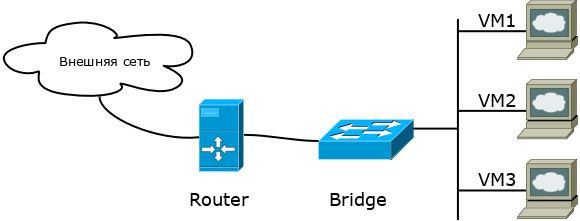
\includegraphics[height=0.4\textheight]{../../slides/networking/net-practice.png}


	\begin{block}{Задача}
		Запустить 3 идентичные виртуальные машины.\\
		Каждой машине назначить адрес из отдельного IP диапазона.\\
		Организовать сетевую ''видимость'' между виртуальными машинами, а также хостом.		
	\end{block}

\end{frame}



\begin{frame}{Практика: создание тестовой среды}
	\begin{block}{Подготовка дисковой подсистемы}
			\begin{itemize}
				\item Создать пустой файл размером в 1.5 GB и отобразить на устройство
					/dev/loop ({\tt dd, losetup})
				\item Создать группу томов на базе этого устройства ({\tt pvcreate, vgcreate})
				\item Выделить 1 GB под логический диск ({\tt lvcreate})
				%\item Скопировать образ виртуального диска в полученный логический том ({\tt dd})
				%\item Создать снимок логического тома на 100MB ({\tt lvcreate}) для каждой виртуальной машины.
			\end{itemize}
	\end{block}
\end{frame}

\begin{frame}{Практика: создание тестовой среды}

	\begin{block}{Запуск виртуальных машин}

		\begin{itemize}
			\item {\tt modprobe kvm-intel} 
			\item {\tt modprobe tun}
			\item Установить centos-minimal на  машину из iso файла.
                        \item Создать два снимка логического тома виртуальной машины
			\item Убедиться в наличии tap интерфейсов
		\end{itemize}
	\end{block}

\end{frame}


\begin{frame}{Практика: создание тестовой среды}

	\begin{block}{Настройка сети на хосте}
			\begin{itemize}
				\item Создать мост {\tt brctl} и назначить ему адреса из соответствующих диапазонов {\tt ifconfig/ip}
				\item Поднять виртуальные интерфейсы {\tt ifconfig/ip}
				\item Добавить виртуальные интерфейсы к мосту {\tt brctl}
			\end{itemize}
	\end{block}
\end{frame}


\begin{frame}{Практика: создание тестовой среды}
	\begin{block}{Настройка сети на виртуальных машинах}
			\begin{itemize}
				\item Назначить адрес устройству eth0 {\tt ifconfig/ip}
				\item Добавить адрес маршрутизатора по умолчанию {\tt route/ip}
				\item Проверить доступность виртуальных машин и хоста {\tt ping/nmap}
			\end{itemize}
	\end{block}
\end{frame}

\begin{frame}{Практика: создание тестовой среды}

	\begin{block}{Настройка роутинга и NAT}
			\begin{itemize}
				\item Разрешить форвардинг на хосте
				\item Настроить NAT на хосте ({\tt iptables},  правило {\tt MASQUERADE})
				\item Проверить доступность хостов из ''внешней'' сети {\tt ping/nmap}
			\end{itemize}
	\end{block}
\end{frame}


